% This file was created by matlab2tikz.
%
%The latest updates can be retrieved from
%  http://www.mathworks.com/matlabcentral/fileexchange/22022-matlab2tikz-matlab2tikz
%where you can also make suggestions and rate matlab2tikz.
%
\definecolor{mycolor1}{rgb}{0.00000,0.44700,0.74100}%
\definecolor{mycolor2}{rgb}{0.85000,0.32500,0.09800}%
%
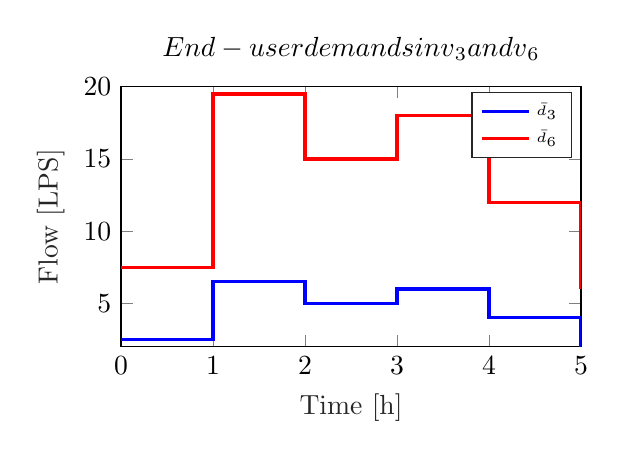
\begin{tikzpicture}

\begin{axis}[%
width=2.3in,
height=1.3in,
at={(0.758in,0.481in)},
scale only axis,
xmin=0,
xmax=5,
xlabel style={font=\color{white!15!black}},
xlabel={Time [h]},
ymin=2,
ymax=20,
ylabel style={font=\color{white!15!black}},
ylabel={Flow [LPS]},
axis background/.style={fill=white},
title style={},
title={$\text{End-user demands in v}_\text{3}\text{ and v}_\text{6}$},
%xmajorgrids,
%ymajorgrids,
legend style={legend cell align=left, align=left, draw=white!15!black}
]
\addplot[const plot, color=blue, line width=1.2pt] table[row sep=crcr] {%
0	2.5\\
1	6.5\\
2	5\\
3	6\\
4	4\\
5	2\\
};
\addlegendentry{\tiny $\bar{d}_3$}

\addplot[const plot, color=red, line width=1.2pt] table[row sep=crcr] {%
0	7.5\\
1	19.5\\
2	15\\
3	18\\
4	12\\
5	6\\
};
\addlegendentry{\tiny $\bar{d}_6$}

\end{axis}
\end{tikzpicture}%